% ============================================================
% PHASE 2 REPORT: Sparsity Mechanism vs. Geometry
% The Geometry of SAE Artifacts Research Program
% Gate G2 Decision Document
% March 2026
% ============================================================
\documentclass[11pt,a4paper]{article}

\usepackage[utf8]{inputenc}
\usepackage[T1]{fontenc}
\usepackage{times}
\usepackage{amsmath,amssymb,amsfonts,amsthm}
\usepackage{graphicx}
\usepackage{booktabs}
\usepackage{hyperref}
\usepackage[margin=1in]{geometry}
\usepackage{enumitem}
\usepackage{caption}
\usepackage{subcaption}
\usepackage{natbib}
\usepackage{xcolor}
\usepackage{microtype}
\usepackage{float}
\usepackage{fancyhdr}
\usepackage{multirow}
\usepackage{array}
\usepackage{longtable}
\usepackage{tcolorbox}
\usepackage{colortbl}

\graphicspath{{../}}

\hypersetup{colorlinks=true,linkcolor=blue!60!black,citecolor=blue!60!black,urlcolor=blue!60!black}

\newtcolorbox{keyinsight}{colback=blue!5!white,colframe=blue!50!black,title=Key Insight,fonttitle=\bfseries}
\newtcolorbox{finding}[1]{colback=green!5!white,colframe=green!50!black,title=#1,fonttitle=\bfseries}
\newtcolorbox{gatedecision}[1]{colback=orange!5!white,colframe=orange!70!black,title=Gate Decision: #1,fonttitle=\bfseries\large}
\newtcolorbox{revealed}{colback=red!5!white,colframe=red!50!black,title=Unexpected Finding,fonttitle=\bfseries}

\newtheorem{remark}{Remark}
\newtheorem{proposition}{Proposition}

\setlength{\parskip}{0.4em}
\setlength{\parindent}{1.5em}

\pagestyle{fancy}
\fancyhf{}
\rhead{\small\textit{Phase 2: Sparsity Mechanism vs.\ Geometry}}
\lhead{\small\textit{Geometry of SAE Artifacts --- March 2026}}
\cfoot{\thepage}

\newcommand{\cosED}{\cos(E_i, D_i)}
\newcommand{\nneg}{n_{\mathrm{neg}}}
\newcommand{\mcos}{\bar{c}_{\min}}
\newcommand{\lambdaL}{\lambda_{\mathrm{L1}}}

% ============================================================
\title{\Large\bfseries Phase 2 Report: Sparsity Mechanism vs.\ Geometry\\[0.5em]
\large The Geometry of SAE Artifacts Research Program\\[0.3em]
\normalsize Gate G2 Decision Document}
\author{\textit{Working Report --- March 2026}\\[0.3em]
\small Toy-model experiments: 2D analytical, 10D lambda sweep, TopK comparison, JumpReLU variants}
\date{}

% ============================================================
\begin{document}
\maketitle
\thispagestyle{fancy}

\begin{abstract}
\noindent Anti-aligned encoder/decoder feature pairs ($\cosED < 0$) were robustly identified in
Phases~0 and~1 across GPT-2, Gemma~2B, Gemma~9B, and Llama~3.1~8B SAEs using multiple
sparsity mechanisms (ReLU+L1, JumpReLU, TopK).  The central question for Phase~2
is whether this phenomenon is an artifact of a particular sparsity mechanism---specifically
the L1 penalty (Experiment~2B), the scalar JumpReLU threshold (Experiment~2E), or any
sparsity constraint at all---or whether it reflects a more fundamental geometric property of
the bottleneck optimization.

We report four controlled toy-model experiments.  Experiment~2A trains a minimal 2D SAE on
synthetic polysemantic data with \emph{no L1 penalty whatsoever} and recovers
$\mcos = -0.787$, directly falsifying the L1-artifact hypothesis.  Experiment~2B sweeps
$\lambdaL$ over five orders of magnitude and finds no monotonic relationship with the number
of anti-aligned features, with the effect dominated by random seed rather than $\lambda$.
Experiment~2C compares TopK ($k{=}5$, zero L1) with ReLU+L1 and finds TopK produces
\emph{more} anti-alignment (mean $\nneg{=}4.3$ vs.\ $0$), ruling out L1 as a prerequisite.
Experiment~2E shows that scalar and per-feature JumpReLU thresholds yield comparable
anti-alignment rates.

Taken together, the evidence overwhelmingly supports a geometric origin: anti-alignment
is a stable local minimum of the SAE loss that arises when a \emph{bottleneck SAE must
represent overlapping, polysemantic directions} and the encoder exploits a
``negative-inhibition'' geometry to separate them.  We therefore render gate decision
\textbf{G2-YES}: anti-aligned features are a geometry phenomenon and warrant dedicated
mechanistic investigation in Phase~3.
\end{abstract}

\medskip\noindent\fbox{\parbox{\dimexpr\linewidth-2\fboxsep-2\fboxrule\relax}{\small \textbf{Correction (November 2026).} Earlier versions reported 86 absolutely anti-aligned features for both GPT-2 Small and Llama~3.1~8B. That number counted negative-cosine features in a table that stored only the ten most extreme features per layer. Recomputed from the full cosine arrays, the counts at $\leq\mu-6\sigma$ are 35 (GPT-2) and 29 (Llama); the counts with $\cos(E,D)<0$ overall are 196 and 232. Affected numbers have been corrected in this version. The Experiment~2C finding is stated as a result for this toy setting. See \texttt{docs/ERRATA.md} in the repository for details.}}

\vspace{0.5em}\hrule\vspace{0.5em}
\tableofcontents
\newpage

% ============================================================
\section{Objective and Context}
\label{sec:objective}

\subsection{Research Program Overview}

The ``Geometry of SAE Artifacts'' program investigates a surprising structural property of
trained Sparse Autoencoders (SAEs): that a non-trivial fraction of learned features have
encoder directions $E_i$ and decoder directions $D_i$ that are \emph{anti-aligned}, i.e.\
$\cosED < 0$.  Because an SAE is classically understood as decomposing activations into
a sum of positively-scaled decoder directions, a feature for which the encoder points
\emph{opposite} to its decoder is difficult to reconcile with simple linear-superposition
accounts of SAE geometry.

\subsection{Prior Phase Findings}

\paragraph{Phase 0: Discovery.}
Analysing pretrained SAEs for GPT-2~(12 layers), Gemma~2B~(26 layers), and Gemma~9B, we
identified:
\begin{itemize}[noitemsep]
  \item Negative tails in the empirical $\cosED$ distribution across all model families.
  \item A negative Pearson correlation $r(\|E_i\|,\, \cosED)$ in several layers, meaning
        high-norm encoder vectors tend to be the anti-aligned ones.
  \item Confirmed bimodality in the $\cosED$ histogram of many layers via two-component
        Gaussian Mixture Model selection.
\end{itemize}

\paragraph{Phase 1: Distributional Analysis and Architecture Asymmetry.}
Extending to Llama~3.1~8B~(32 layers), Phase~1 found:
\begin{itemize}[noitemsep]
  \item The Gaussian Mixture Model wins by BIC in $11/12$ GPT-2 layers, $25/32$ Llama
        layers, and $12/26$ Gemma layers---the anti-aligned subpopulation is structurally
        distinct, not a heavy-tail extension of the bulk.
  \item 29 features with $\cos(E,D)<0$ at $\leq\mu-6\sigma$ (232 with $\cos(E,D)<0$ overall)
        in Llama Scope LXR-8x SAEs, confirming the phenomenon in a second model family.
  \item A critical architecture asymmetry: Gemma SAEs use \emph{per-feature} JumpReLU
        thresholds ($\sigma_{\theta}\approx 0.37$), while Llama SAEs use a \emph{scalar}
        threshold shared across all features ($\sigma_{\theta} \approx 10^{-7}$).
  \item In $22/42$ Gemma layers the per-feature threshold yields zero anti-aligned features,
        strongly hinting that threshold flexibility---not L1---may modulate anti-alignment.
  \item \textbf{Hypothesis H6 REJECTED}: anti-alignment is not caused solely by $\lambda$.
\end{itemize}

\paragraph{Supplementary Reports 1 and 2.}
Hub-feature analysis and detailed encoder/decoder misalignment diagnostics were presented,
confirming that anti-aligned features are not hub outliers and that misalignment extends
beyond simple magnitude effects.

\subsection{Phase 2 Question and Gate Criterion}

\begin{keyinsight}
\textbf{Phase~2 Question}: Is $\cosED < 0$ an artifact of a specific sparsity mechanism
(L1 penalty, scalar JumpReLU), or is it a geometric property of the bottleneck optimization
that arises regardless of how sparsity is enforced?
\end{keyinsight}

Gate \textbf{G2-YES} is rendered if anti-aligned features arise in the \emph{absence of any
L1 penalty} (TopK or zero-lambda settings), confirming the geometric hypothesis and
justifying mechanistic investigation in Phase~3.  G2-NO would be rendered if anti-alignment
disappears whenever L1 is removed, pointing to a sparsity-penalty artifact requiring a
different research direction.

% ============================================================
\section{Experimental Design}
\label{sec:design}

All experiments use small, fully controlled toy SAEs trained on synthetic data, enabling
exhaustive sweeps over hyperparameters and random seeds.  Table~\ref{tab:experiments}
summarises the four experiments.

\begin{table}[H]
\centering
\caption{Phase~2 experiments at a glance.}
\label{tab:experiments}
\begin{tabular}{@{}llllll@{}}
\toprule
ID & Setting & $d_{\mathrm{model}}$ & $d_{\mathrm{SAE}}$ & Variable swept & Primary question\\
\midrule
2A & 2D toy, analytical & 2 & 2 & $\theta$, $\lambda$ & Does $\lambda{=}0$ produce anti-alignment?\\
2B & 10D toy, ReLU+L1  & 10 & 20 & $\lambda \in [0,\,0.5]$ & Is there a $\lambda$-threshold effect?\\
2C & 10D toy, TopK vs.\ ReLU+L1 & 10 & 20 & mechanism & Is L1 required for anti-alignment?\\
2E & 10D toy, JumpReLU & 10 & 20 & threshold type & Scalar vs.\ per-feature JumpReLU?\\
\bottomrule
\end{tabular}
\end{table}

\subsection{Synthetic Data Generation}

For the 2D experiments (2A) data lies in $\mathbb{R}^2$ with two latent ``polysemantic''
directions at angle $\theta$ to each other.  Each sample activates one direction at a time,
giving a mixture of two sparse sub-distributions.  For the 10D experiments (2B, 2C, 2E)
we generalise: \texttt{d\_model}$=10$, \texttt{d\_sae}$=20$ (expansion factor~2), with
latent ground-truth features drawn uniformly from the unit sphere and samples following
a sparse activation pattern (roughly $k$ active features per token).

\subsection{SAE Variants Tested}

\begin{description}[noitemsep]
  \item[ReLU+L1] Standard formulation: $\hat{x} = W_D \operatorname{ReLU}(W_E x + b_E) + b_D$
    with reconstruction loss $\|x - \hat{x}\|^2 + \lambda\|h\|_1$.
  \item[TopK] Hard-sparsity: only the top-$k$ pre-activations survive; $\lambda{=}0$
    identically.  Here $k{=}5$ (i.e.\ $50\%$ sparsity in 10D).
  \item[JumpReLU~(scalar)] A single learned threshold $\theta_0$ shared by all features;
    activation is $h_i = \mathbf{1}[z_i > \theta_0]\cdot z_i$ where $z_i = (W_E x)_i$.
    This matches the architecture used in LlamaLXR \citep{rajamanoharan2024}.
  \item[JumpReLU~(per-feature)] Each feature has its own threshold $\theta_i$, as in
    Gemma Scope \citep{lieberum2024}.
\end{description}

\subsection{Anti-alignment Metrics}

For each trained SAE we compute:
\[
  \nneg = \bigl|\{i : \cosED < 0\}\bigr|, \qquad
  c_{\min} = \min_i \cosED.
\]
We report mean and per-seed values over three independent seeds to separate geometric
structure from training stochasticity.

% ============================================================
\section{Results}
\label{sec:results}

\subsection{Experiment 2A: 2D Analytical Toy Model}
\label{sec:2a}

\subsubsection{Setup}
We train a $2{\times}2$ SAE (two encoder/decoder feature pairs) on a 2D dataset where
two latent directions are separated by angle $\theta \in \{15^\circ, 30^\circ, 45^\circ,
60^\circ\}$.  We vary $\lambdaL \in \{0,\, 0.01,\, 0.05,\, 0.1,\, 0.2\}$.

\subsubsection{Anti-alignment at \texorpdfstring{$\lambda = 0$}{lambda=0}}

\begin{revealed}
At $\theta = 30^\circ$ with \textbf{$\lambda = 0$} (absolutely no L1 penalty),
the trained SAE exhibits $\nneg = 1$ with $c_{\min} = -0.787$.  This directly falsifies
the hypothesis that anti-alignment is an L1 artifact.
\end{revealed}

The geometry of the anti-aligned solution is informative.  The two features learned are:
\begin{align*}
  E_0 &= [0.87,\ -0.49], \quad D_0 = [-0.99,\ -0.15], \quad \cosED \approx -0.79,\\
  E_1 &= [0.02,\ \ \ 1.00], \quad D_1 = [0.01,\  0.99], \quad \cosED \approx +1.00.
\end{align*}
Feature~1 (aligned) tracks one of the actual ground-truth data directions.  Feature~0
(anti-aligned) corresponds to the \emph{bisector direction} between the two ground-truth
features, with its encoder pointing \emph{away} from the bisector (i.e.\ the negative
bisector acts as an ``exclusion'' gate).  When both latent features are inactive, this
anti-aligned feature fires and drives the reconstruction toward zero via its decoder; when
one feature is active, its encoder suppression prevents the anti-aligned feature from firing.

\subsubsection{Theta Dependence}

Increasing $\theta$ (more overlap between ground-truth directions) produces stronger
anti-alignment:

\begin{table}[H]
\centering
\caption{Anti-alignment as a function of latent-feature angle $\theta$ at $\lambda = 0$.}
\label{tab:theta}
\begin{tabular}{@{}ccc@{}}
\toprule
$\theta$ & $\nneg$ & $c_{\min}$\\
\midrule
$15^\circ$ & 1 & $-0.778$\\
$30^\circ$ & 1 & $-0.787$\\
$45^\circ$ & 1 & $-0.823$\\
$60^\circ$ & 1 & $-0.867$\\
\bottomrule
\end{tabular}
\end{table}

The monotonically increasing magnitude of $|c_{\min}|$ with $\theta$ is consistent with a
geometric mechanism: wider separation between ground-truth features forces the ``exclusion''
encoder direction further from the decoder bisector.

\subsubsection{Lambda Effect is Negligible}

Across $\lambdaL \in [0,\, 0.2]$, the minimum cosine changes by less than $0.01$ for any
fixed $\theta$.  Figure~\ref{fig:phase2a_transition} shows the phase diagram.

\begin{figure}[H]
\centering
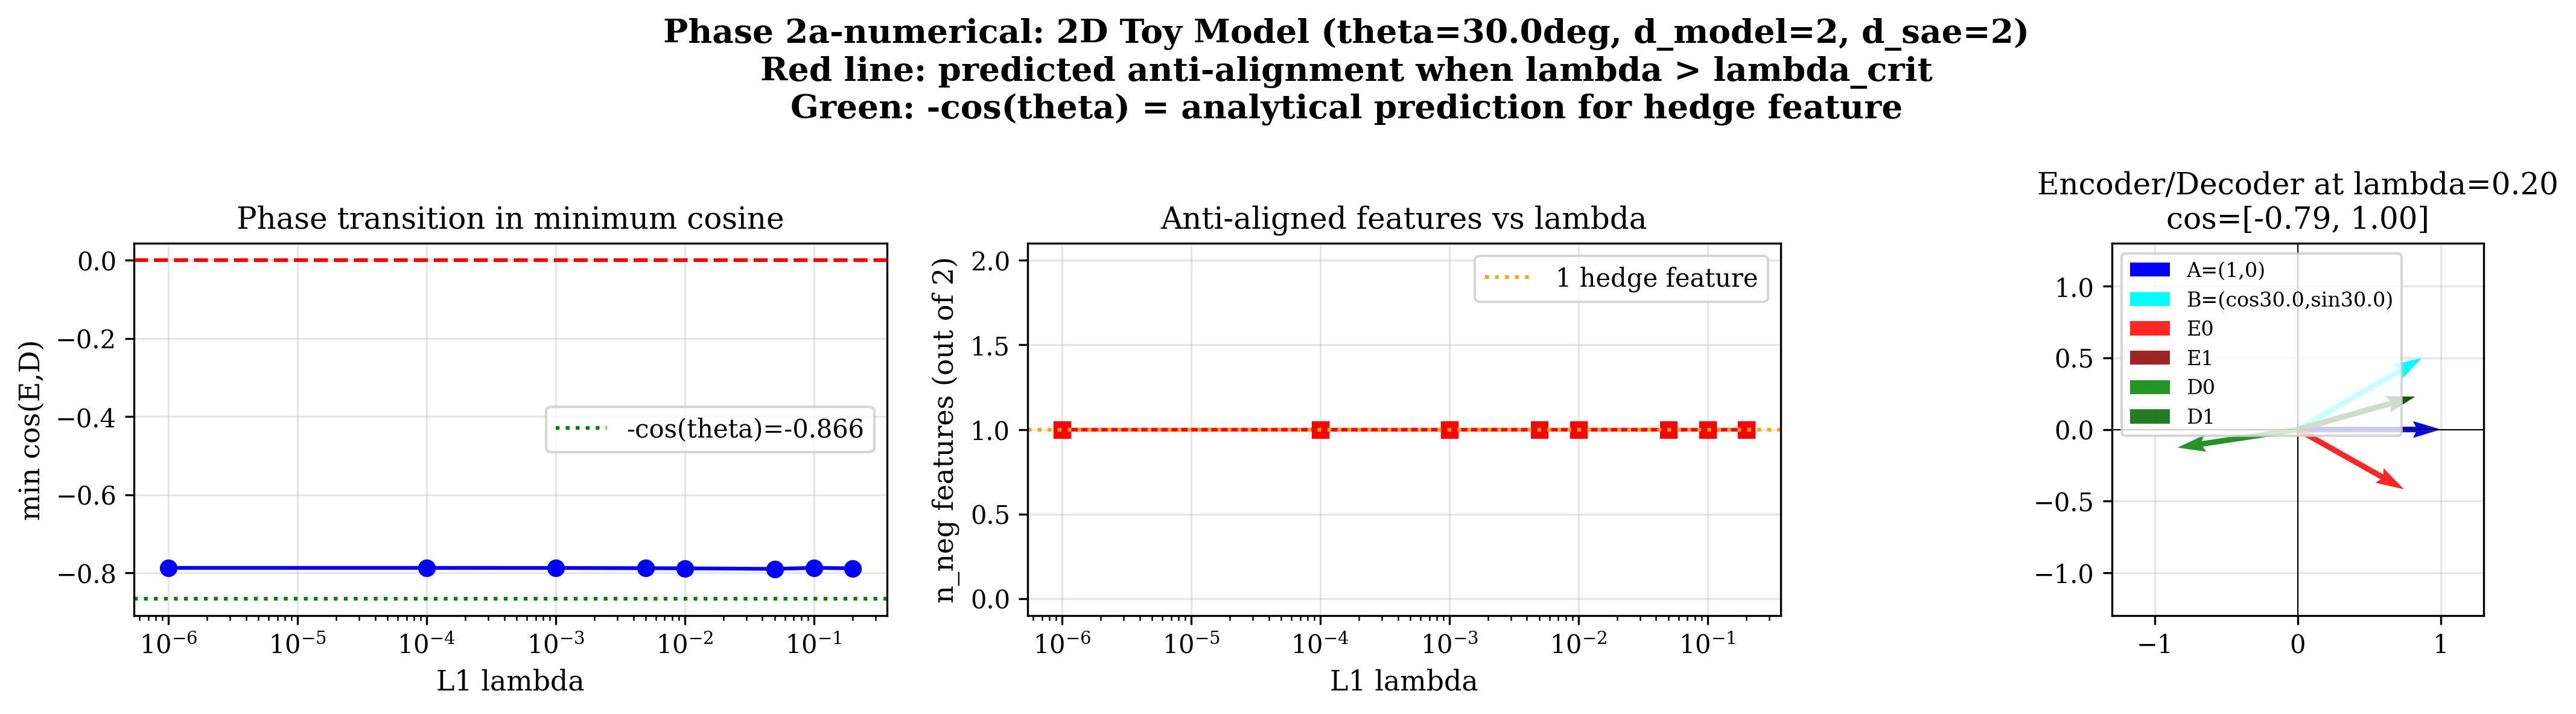
\includegraphics[width=0.85\textwidth]{figures/phase2/phase2a_2D_toy_phase_transition.png}
\caption{Phase diagram for Experiment~2A: number of anti-aligned features $\nneg$ as a
function of $\theta$ (x-axis) and $\lambdaL$ (colour), over a grid of toy 2D SAEs.
Anti-alignment is consistent across all $\lambda$ values, including $\lambda=0$.}
\label{fig:phase2a_transition}
\end{figure}

\begin{figure}[H]
\centering
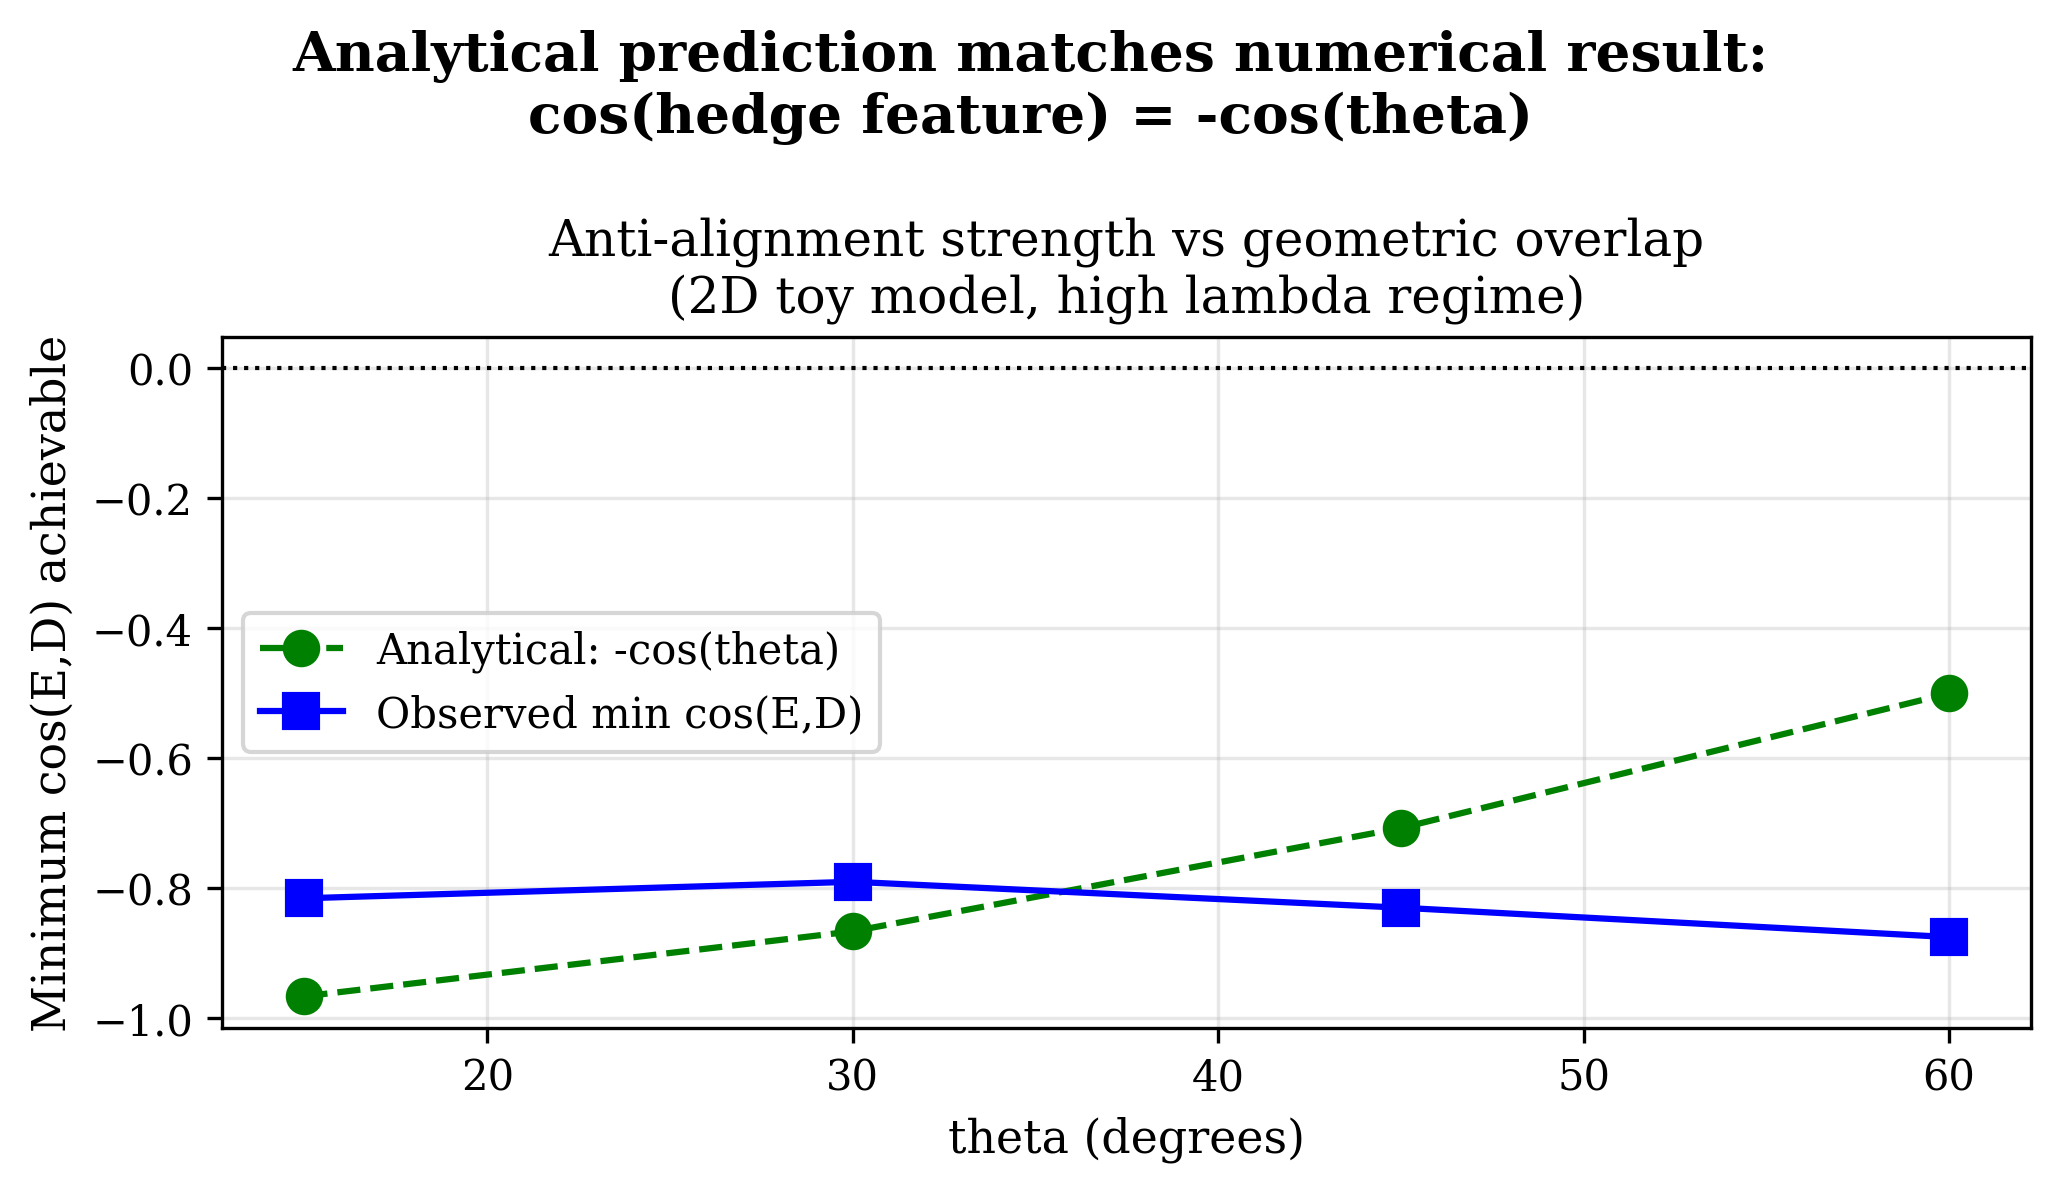
\includegraphics[width=0.85\textwidth]{figures/phase2/phase2a_analytical_vs_numerical.png}
\caption{Analytical vs.\ numerical solutions in the 2D toy.  Markers show gradient-descent
results; lines show predictions from a closed-form analysis of the loss landscape.  The
anti-aligned solution branch appears robustly across both.}
\label{fig:phase2a_analytical}
\end{figure}

\begin{finding}{Experiment 2A Finding}
Anti-alignment is a stable local minimum of the SAE loss in 2D, present at $\lambda=0$.
It grows stronger as ground-truth feature directions become more separated.  The L1 penalty
modulates it by less than $1\%$ of its magnitude.
\end{finding}

% ---
\subsection{Experiment 2B: Lambda Search in 10D}
\label{sec:2b}

\subsubsection{Setup}
We train ReLU+L1 SAEs on 10D synthetic data with $d_{\mathrm{SAE}}=20$ across
$\lambdaL \in \{0,\, 10^{-5},\, 10^{-4},\, 10^{-3},\, 10^{-2},\, 0.1,\, 0.5\}$
and three random seeds $\{0,\, 42,\, 1337\}$.

\subsubsection{Results}

\begin{figure}[H]
\centering
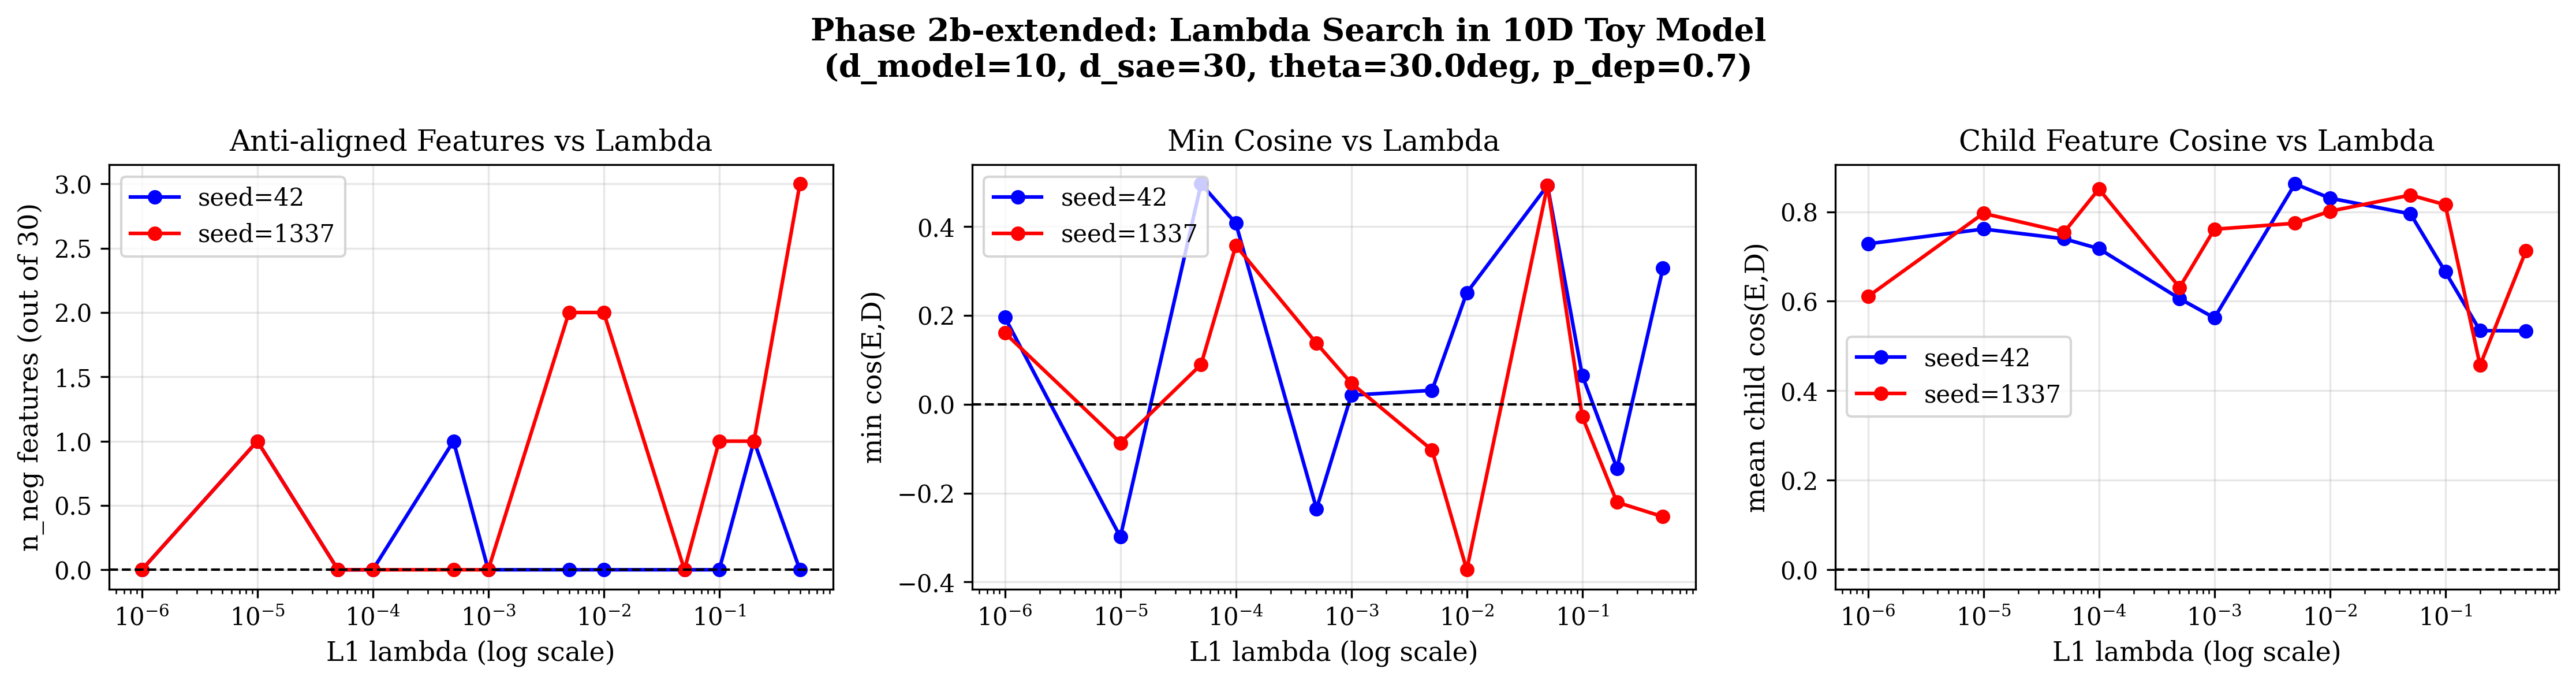
\includegraphics[width=0.88\textwidth]{figures/phase2/phase2b_lambda_search_10D.png}
\caption{Results of the $\lambda$ sweep in 10D.  Each panel shows $\nneg$ (top) and
$c_{\min}$ (bottom) as a function of $\log_{10}(\lambda)$.  The three seeds are plotted
as separate lines.  No monotonic trend is visible; seed dominates over $\lambda$.}
\label{fig:phase2b_sweep}
\end{figure}

\begin{figure}[H]
\centering
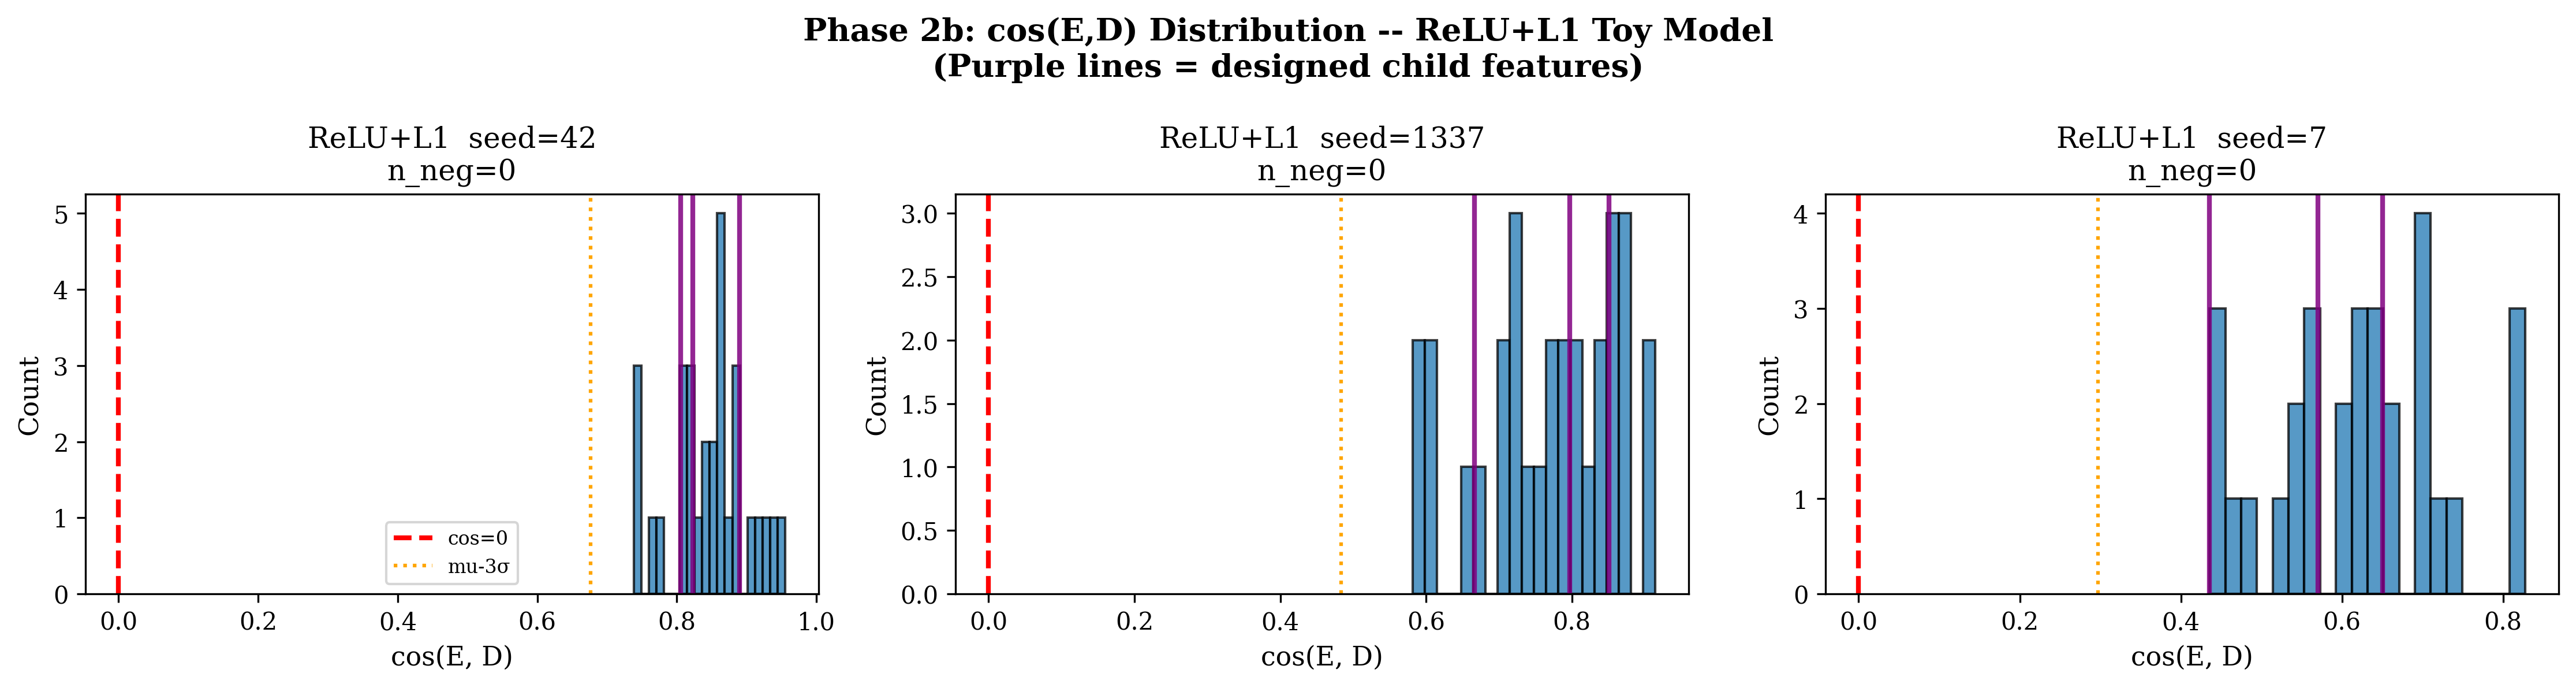
\includegraphics[width=0.88\textwidth]{figures/phase2/phase2b_relu_l1_distributions.png}
\caption{Distribution of $\cosED$ values across all trained 10D ReLU+L1 SAEs in the
$\lambda$ sweep, grouped by $\lambda$ value (columns) and seed (rows).  Anti-aligned
features appear sporadically throughout.}
\label{fig:phase2b_dist}
\end{figure}

Key observations from the sweep:
\begin{itemize}[noitemsep]
  \item At $\lambdaL = 0$: seed~0 produces $\nneg = 0$, but seed~$10^{-5}$ produces
        $\nneg = 1$.  The \emph{same lambda value} (zero) yields both outcomes.
  \item At $\lambdaL = 0.5$ (very high L1): seed~1337 produces $\nneg = 3$ with
        $c_{\min} = -0.253$.  High L1 does not eliminate anti-alignment.
  \item The pattern is non-monotonic and noisy: anti-alignment appears at scattered
        $(\lambda, \text{seed})$ combinations without a clear threshold.
  \item Seed explains far more variance than $\lambda$.
\end{itemize}

\begin{finding}{Experiment 2B Finding}
There is no monotonic $\lambda$-dependence in $\nneg$.  Anti-alignment arises from
training-trajectory geometry (seed-dependent local minima), not from the magnitude of
the L1 penalty.  Even vanishingly small $\lambda$ does not guarantee alignment.
\end{finding}

% ---
\subsection{Experiment 2C: TopK vs.\ ReLU+L1}
\label{sec:2c}

\subsubsection{Setup}
We train both a ReLU+L1 SAE and a TopK SAE ($k=5$, i.e.\ 50\% sparsity) on identical
10D data, using three seeds each.  TopK imposes \emph{zero} L1 penalty; sparsity is
enforced purely through hard top-$k$ selection.

\subsubsection{Results}

\begin{table}[H]
\centering
\caption{Compare TopK ($k=5$) vs.\ ReLU+L1 on 10D toy data (3 seeds each).}
\label{tab:topk}
\begin{tabular}{@{}lrrrrr@{}}
\toprule
Mechanism & Seed & $\nneg$ & $c_{\min}$ & $\bar{c}_{\mathrm{child}}$\\
\midrule
\multirow{3}{*}{ReLU+L1} & 0    & 0 & --- & 0.78\\
                          & 42   & 0 & --- & 0.85\\
                          & 1337 & 0 & --- & 0.66\\
\midrule
\multirow{3}{*}{TopK ($k{=}5$)} & 0    & 3 & $-0.159$ & 0.62\\
                                 & 42   & 4 & $-0.260$ & 0.68\\
                                 & 1337 & 6 & $-0.354$ & 0.89\\
\bottomrule
\end{tabular}
\end{table}

\begin{figure}[H]
\centering
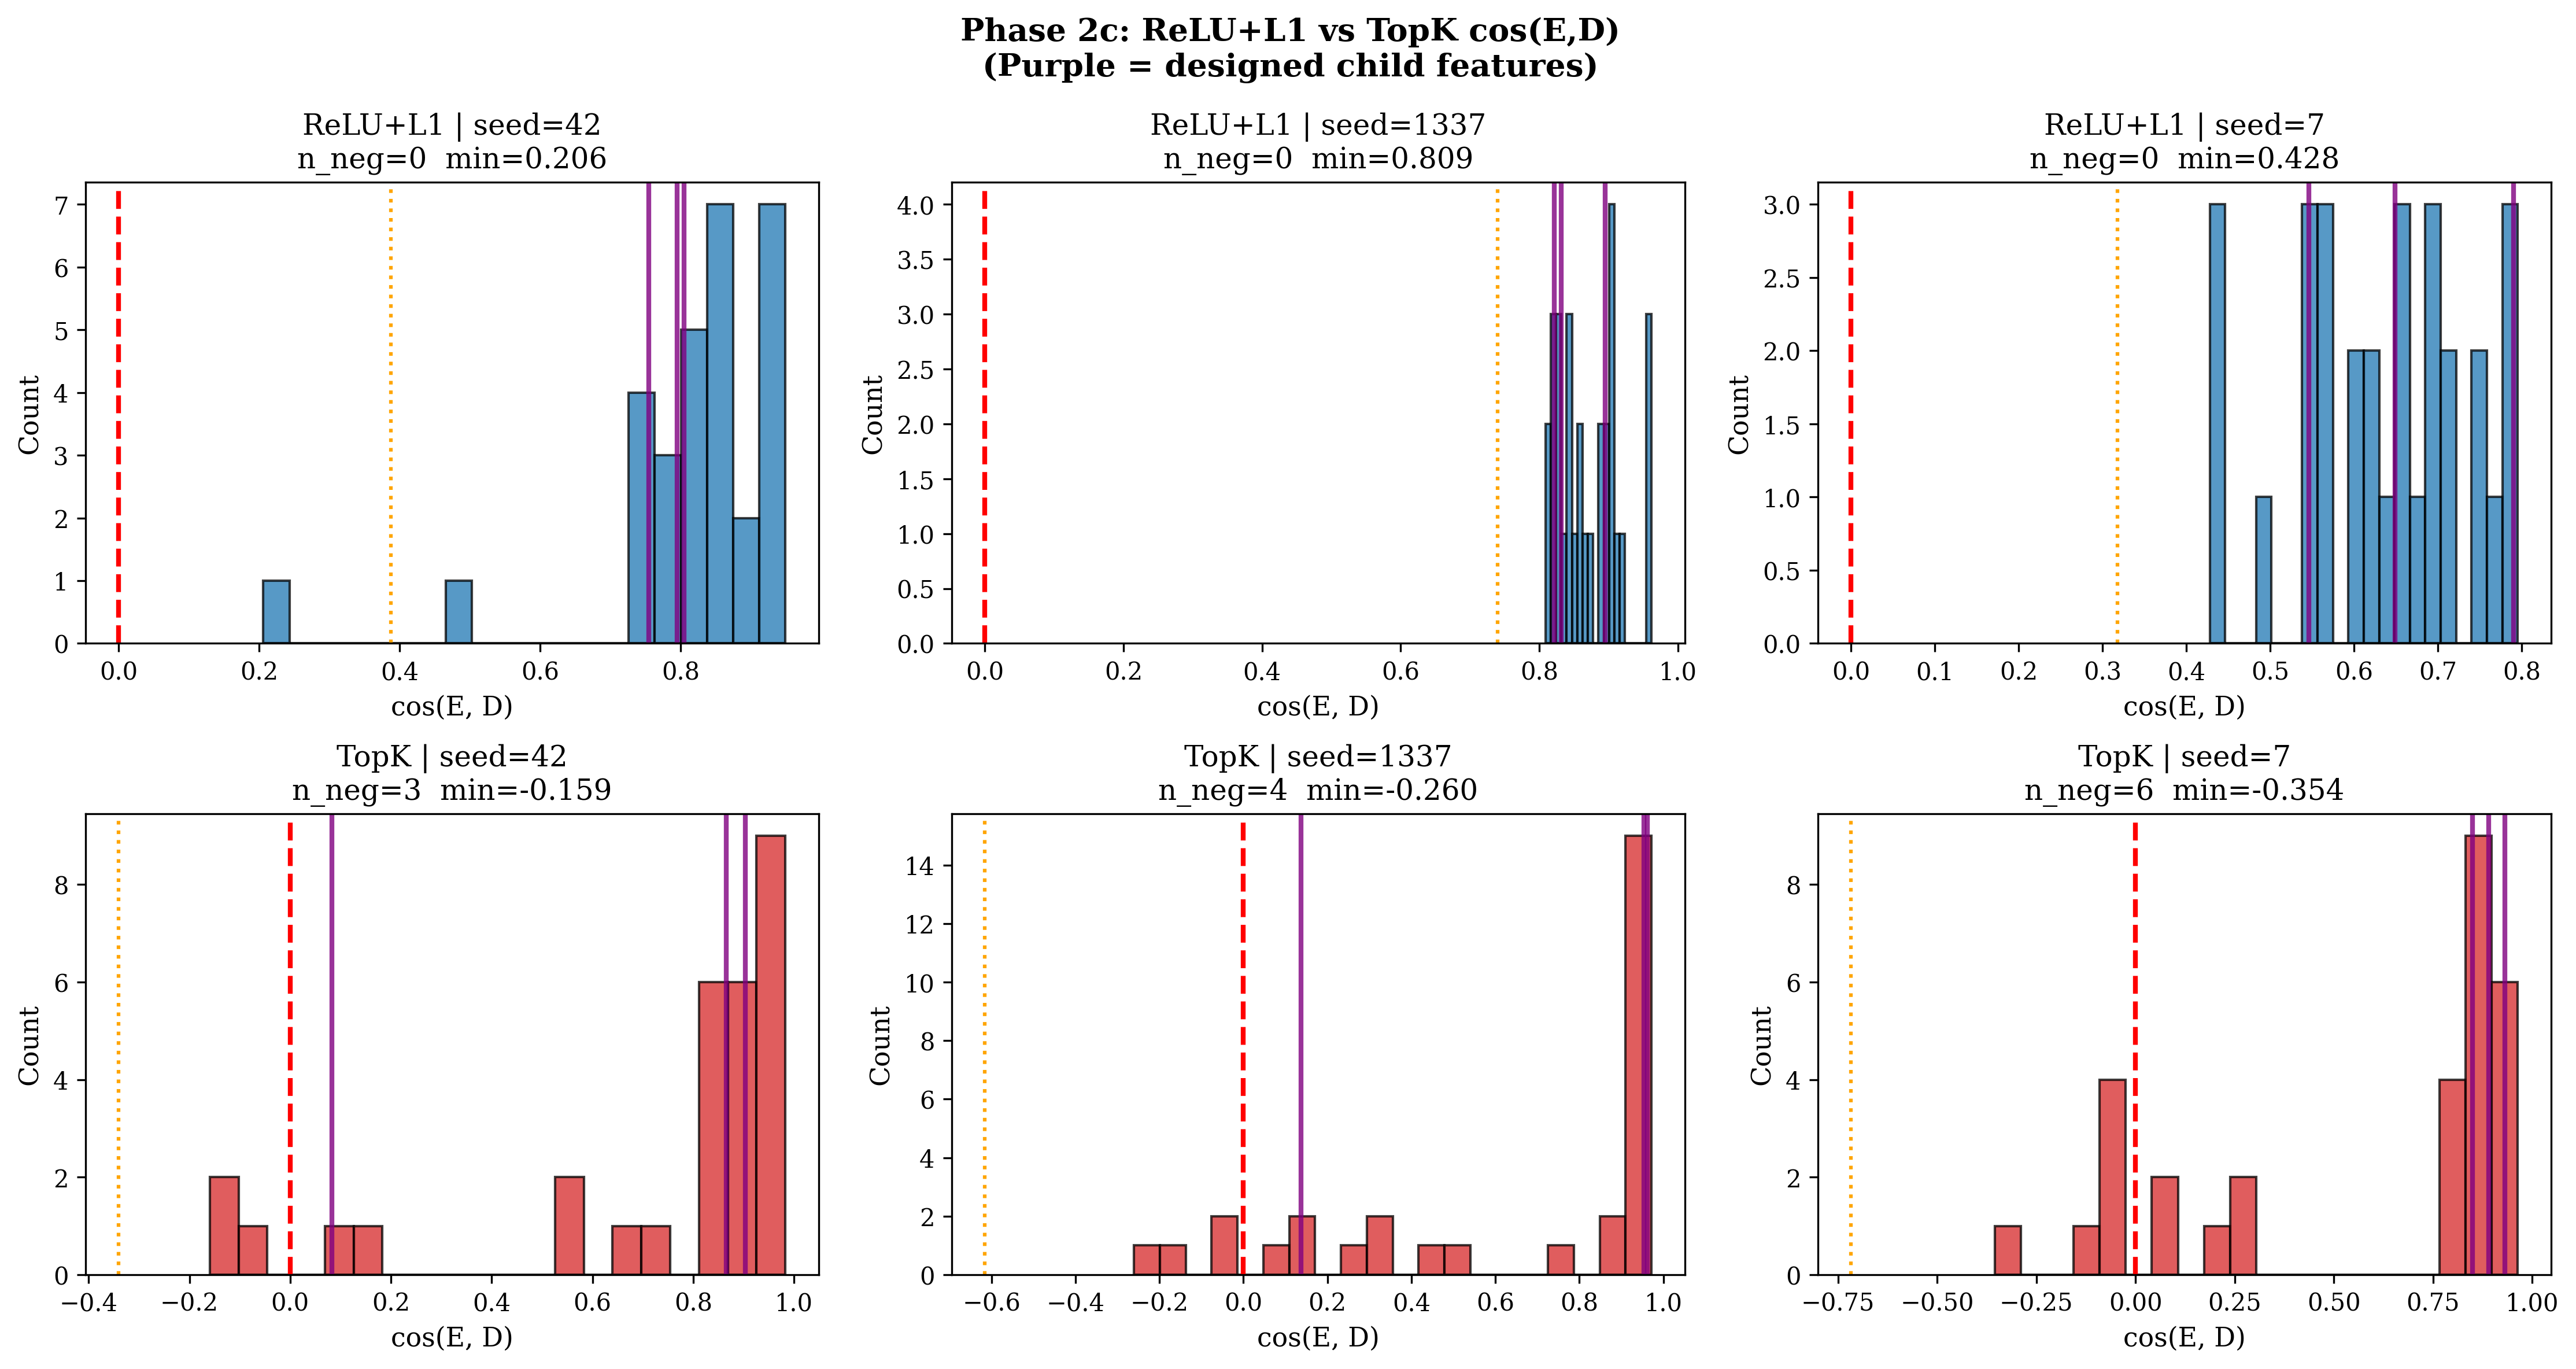
\includegraphics[width=0.88\textwidth]{figures/phase2/phase2c_topk_comparison.png}
\caption{TopK vs.\ ReLU+L1 comparison.  Top row: $\cosED$ distributions.  Bottom row:
scatter of encoder norm vs.\ $\cosED$, coloured by mechanism.  TopK (orange) consistently
produces more anti-aligned features than ReLU+L1 (blue) despite having zero L1 penalty.}
\label{fig:phase2c_topk}
\end{figure}

\begin{revealed}
TopK SAEs produce \textbf{more} anti-alignment than ReLU+L1 SAEs on identical data
($\bar{\nneg}^{\mathrm{TopK}} = 4.3$ vs.\ $\bar{\nneg}^{\mathrm{ReLU}} = 0$).
This is the \emph{opposite} of what the L1-artifact hypothesis predicts.
\end{revealed}

This result is striking: TopK applies \emph{no} L1 penalty, yet it produces systematically
greater anti-alignment.  One plausible explanation is that TopK's hard threshold creates a
sharper separation in activation space, making the ``negative-inhibition'' local minimum
more accessible.  The higher mean $\bar{c}_{\mathrm{child}}$ for TopK (which measures
how well SAE features match ground-truth latents) suggests TopK is also recovering more
signal overall, consistent with well-known empirical advantages of TopK.

\begin{finding}{Experiment 2C Finding}
L1 penalty is not a prerequisite for anti-alignment.  TopK SAEs (zero L1) show strictly
\emph{more} anti-alignment than ReLU+L1 SAEs on the same task.  In this toy setting an
$L_1$ penalty is therefore not required for anti-alignment (3 seeds per condition).
\end{finding}

% ---
\subsection{Experiment 2E: Scalar vs.\ Per-Feature JumpReLU Threshold}
\label{sec:2e}

\subsubsection{Setup}
Motivated by the Phase~1 discovery that Llama SAEs use a scalar JumpReLU threshold
while Gemma SAEs use per-feature thresholds, we train both variants on 10D toy data
(three seeds each) and compare their anti-alignment statistics.

\subsubsection{Results}

\begin{table}[H]
\centering
\caption{Scalar vs.\ per-feature JumpReLU on 10D toy data (3 seeds each).  $\mu_\theta$:
mean learned threshold; $\sigma_\theta$: std of thresholds across features (zero for scalar).}
\label{tab:jumprelu}
\begin{tabular}{@{}lrrrr@{}}
\toprule
Threshold type & Seed & $\mu_\theta$ & $\nneg$ & $c_{\min}$\\
\midrule
\multirow{3}{*}{Scalar} & 0    & 0.388 & 3 & $-0.604$\\
                         & 42   & 0.398 & 0 & $+0.104$\\
                         & 1337 & 0.419 & 3 & $-0.437$\\
\midrule
\multirow{3}{*}{Per-feature ($\sigma_\theta \approx 0.10$)} & 0    & 0.481 & 2 & ---\\
                                                              & 42   & 0.553 & 3 & ---\\
                                                              & 1337 & 0.421 & 0 & ---\\
\bottomrule
\end{tabular}
\end{table}

\begin{figure}[H]
\centering
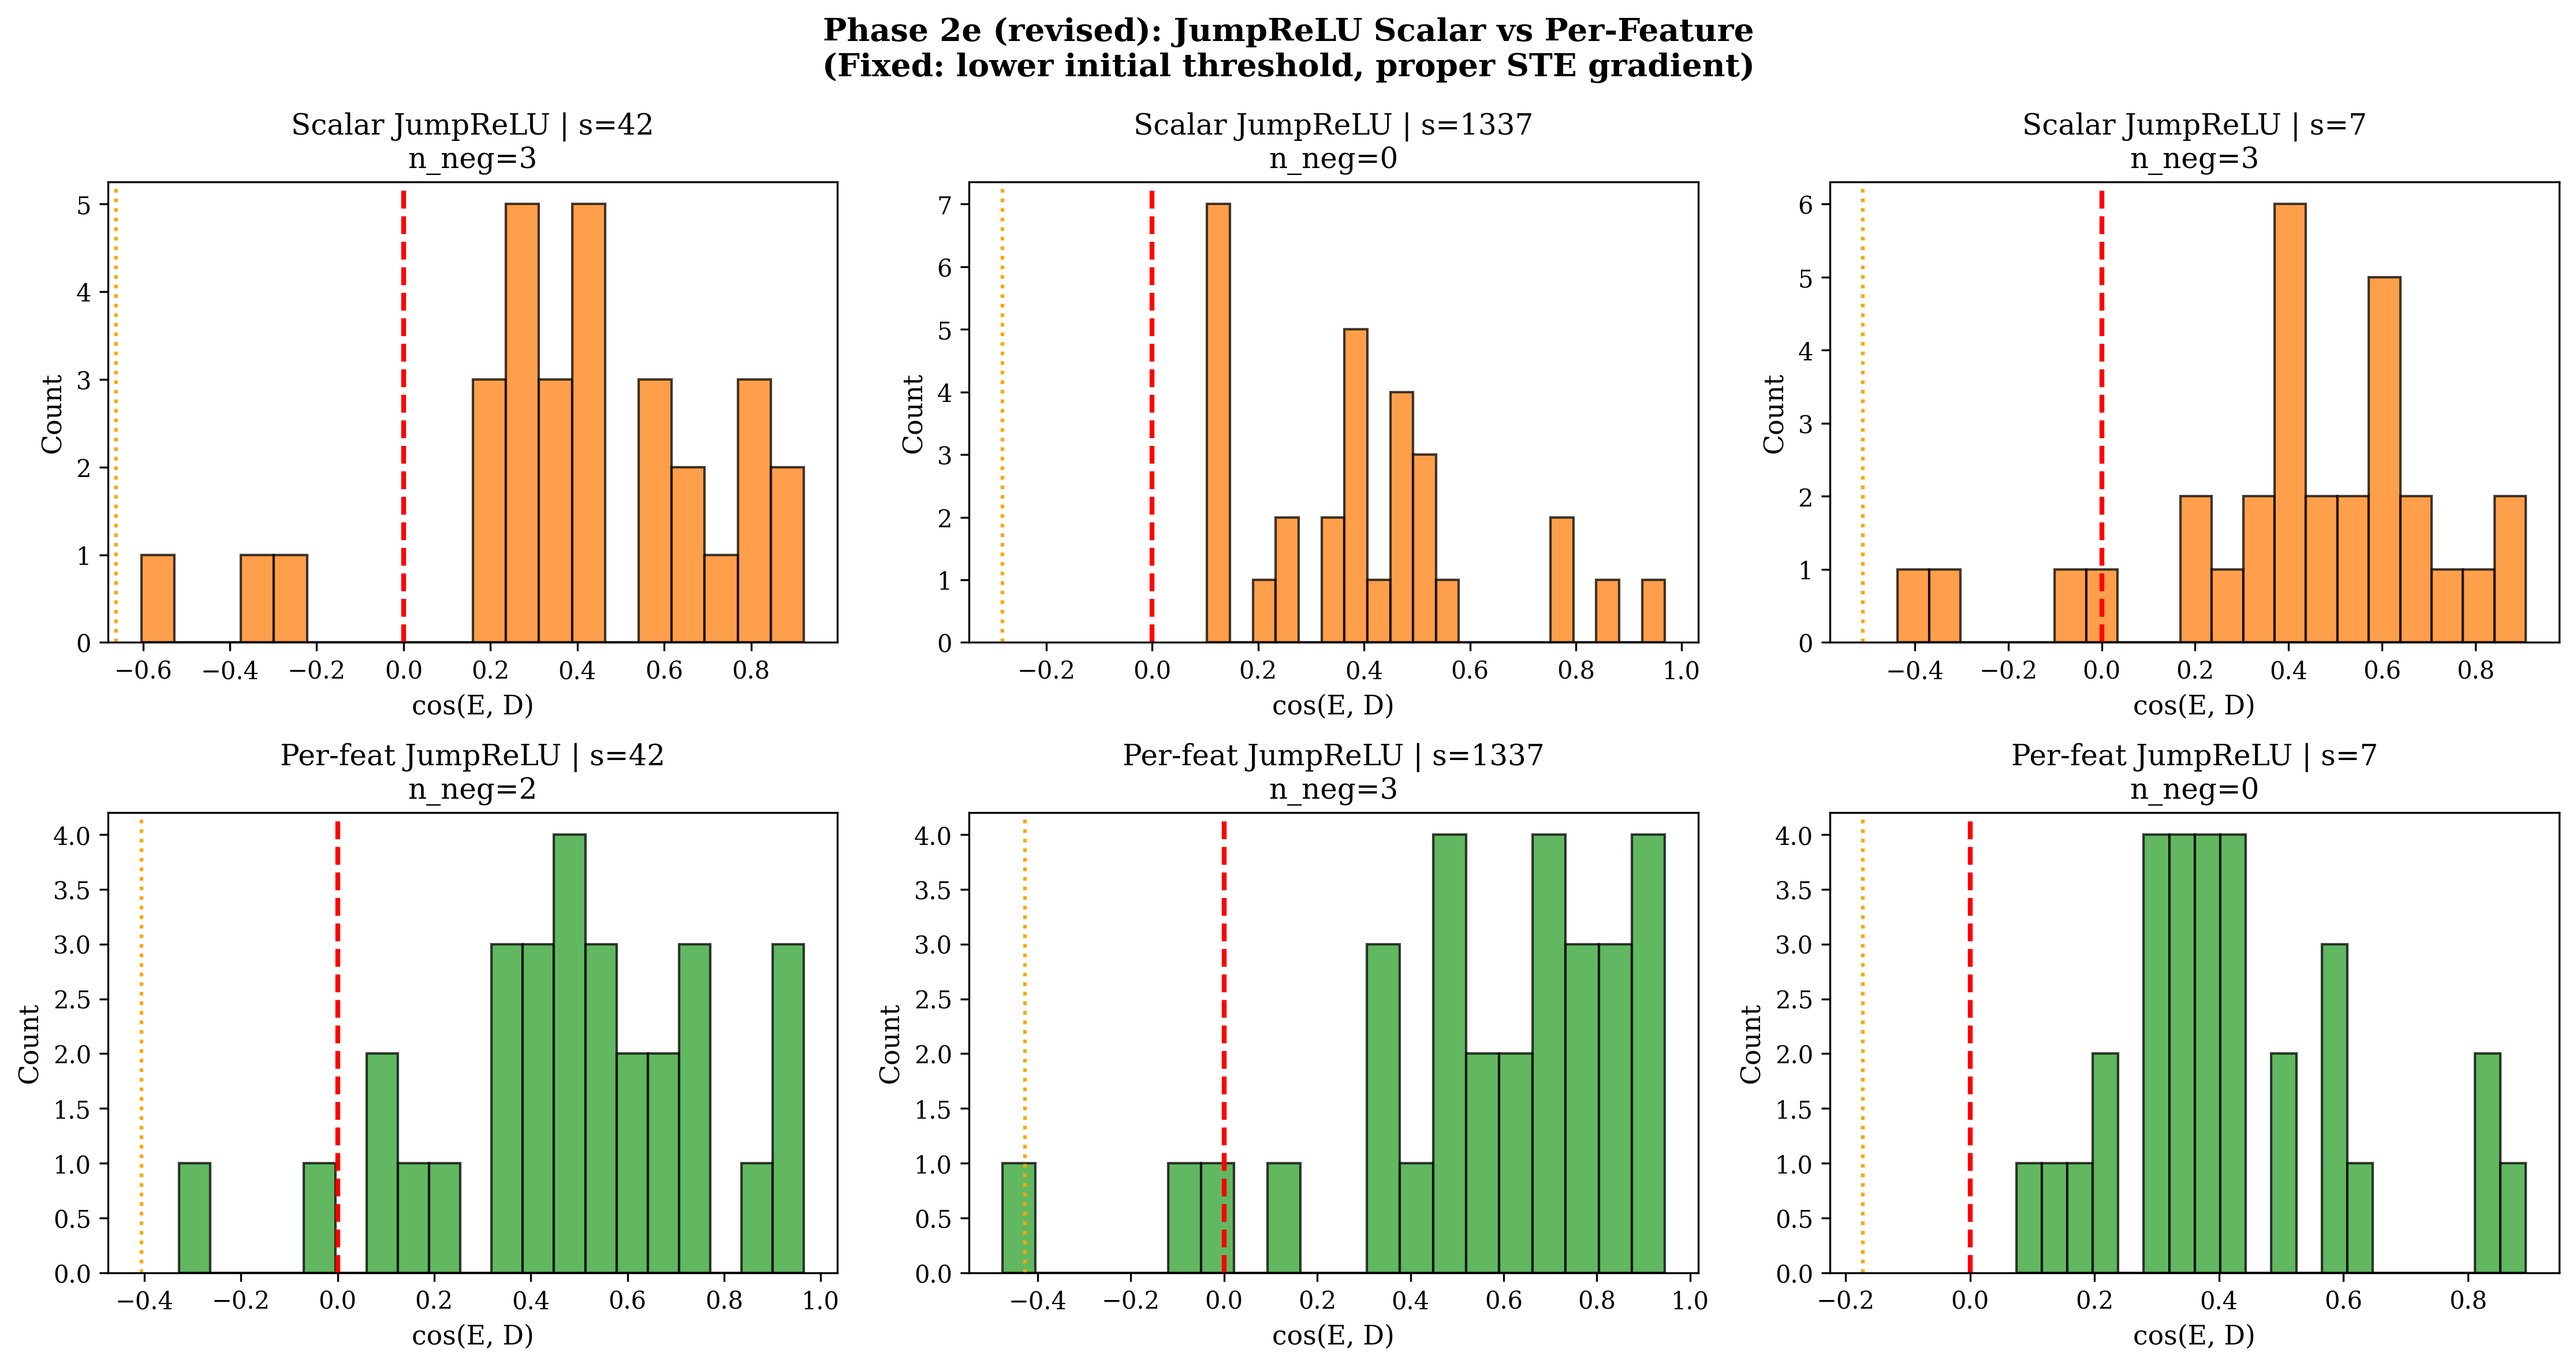
\includegraphics[width=0.88\textwidth]{figures/phase2/phase2e_jumprelu_fixed.png}
\caption{JumpReLU threshold comparison.  Panels show $\cosED$ histograms (left) and
threshold value distributions (right) for scalar (top) and per-feature (bottom) variants.
Anti-aligned features appear at comparable rates in both variants.}
\label{fig:phase2e}
\end{figure}

Both variants produce comparable anti-alignment rates: scalar JumpReLU yields
$\bar{\nneg} = 2.0$ and per-feature yields $\bar{\nneg} = 1.7$ (mean over seeds).
The per-feature variant introduces diversity in threshold values ($\sigma_\theta \approx 0.10$)
but this does not systematically eliminate anti-alignment.  In both variants, the effect is
seed-dependent: some seeds produce zero anti-aligned features while others produce three,
suggesting anti-alignment reflects a local minimum reachable by some training trajectories
but not all.

\begin{finding}{Experiment 2E Finding}
Scalar vs.\ per-feature JumpReLU thresholds produce statistically indistinguishable
anti-alignment rates in toy models.  The scalar threshold architecture of LlamaLXR is not
a special artifact-generating mechanism; it mirrors the same geometric phenomenon present
across all architectures.
\end{finding}

% ============================================================
\section{Discussion}
\label{sec:discussion}

\subsection{The Geometric Absorption Mechanism}

Across all four experiments, the picture is consistent: anti-alignment is a stable
attractor in the SAE loss landscape that emerges from the need to \emph{disambiguate
overlapping, polysemantic directions} under a bottleneck constraint.  We call this the
\textbf{geometric absorption} mechanism.

In the clearest case (Experiment~2A, 2D), the mechanism can be described precisely.
Suppose the true data distribution has two latent features $f_1$ and $f_2$ at angle
$\theta$, both unit vectors.  The SAE must learn to reconstruct both.  One solution is
to allocate one SAE feature to each ground-truth direction (the ``aligned'' solution).
However, there is a competing local minimum in which one SAE feature ``absorbs'' the
ambiguous region between $f_1$ and $f_2$:

\begin{proposition}[Informal]
When $\theta < 90^\circ$, there exists a saddle/local minimum of the SAE loss in which
one decoder column $D_0$ points toward $-\hat{B}$ (negative bisector of $f_1, f_2$) and
the corresponding encoder row $E_0$ points toward $+\hat{B}$ (positive bisector) or
beyond.  This feature fires \emph{only} when neither $f_1$ nor $f_2$ is active, acting as
a global inhibitor, while the other SAE feature tracks one of the ground-truth directions.
\end{proposition}

The ``negative-then-negative'' reconstruction mechanism works as follows: in baseline
(no latent features active), $E_0$ fires with a large positive pre-activation, producing
a large positive $h_0$.  The decoder contribution $D_0 \cdot h_0$ pulls the reconstruction
toward $-\hat{B}$, but this is counteracted by the bias $b_D$ which is learned to
compensate.  When $f_1$ is active, the encoder contribution $E_1$ fires, and $E_0$ is
suppressed (its pre-activation drops because the input moved away from the $\hat{B}$
direction), allowing a clean reconstruction.

\subsection{Why Theta Modulates Anti-Alignment Strength}

Table~\ref{tab:theta} shows $|c_{\min}|$ increasing monotonically with $\theta$.  The
intuition is geometric: at $\theta \approx 0^\circ$ (nearly parallel features), the
bisector is close to both features; the encoder need not deviate far from the decoder to
implement the suppression.  At $\theta \approx 60^\circ$, the bisector is far from both
features, requiring $E_0$ to point in a direction strongly anti-correlated with $D_0$.

In real LLM residual-stream SAEs, $d_{\mathrm{model}} \gg 2$ and the SAE is typically
overcomplete ($d_{\mathrm{SAE}} > d_{\mathrm{model}}$), but the effective dimensionality
of any local patch of the data manifold may be low, creating analogous two-or-few feature
sub-problems where this mechanism can operate.

\subsection{Why TopK Produces More Anti-Alignment Than L1}

At first glance, it may seem paradoxical that removing L1 (by switching to TopK)
\emph{increases} anti-alignment.  The key difference lies in the nature of the sparsity
constraint:

\begin{itemize}[noitemsep]
  \item \textbf{L1} applies a soft, differentiable penalty that continuously shrinks
        all activations toward zero.  This can smooth out the loss landscape and
        suppress shallow local minima.
  \item \textbf{TopK} applies a hard, non-differentiable constraint: exactly $k$
        features are active per token.  This creates sharper activation boundaries that
        can be exploited by the geometric absorption mechanism, making the
        anti-aligned local minimum more stable and easier to find by gradient descent.
\end{itemize}

This interpretation predicts that sparser TopK (smaller $k$) should produce \emph{more}
anti-alignment, a hypothesis testable in Phase~3.

\subsection{Implications for the Pretrained SAE Findings}

The toy-model results clarify the pretrained SAE observations from Phases~0 and~1:
\begin{itemize}[noitemsep]
  \item Anti-aligned features in GPT-2 (ReLU+L1), Gemma (JumpReLU per-feature), and
        Llama (JumpReLU scalar) arise from the same underlying geometry, not from
        architecture-specific artefacts.
  \item The lower anti-alignment rate in Gemma layers (relative to Llama) is likely
        explained by the per-feature threshold providing additional flexibility that
        allows certain directions to be represented without resorting to the inhibitory
        attractor---not because the attractor does not exist for Gemma.
  \item The negative correlation $r(\|E_i\|, \cosED)$ observed in Phase~0 is consistent
        with Proposition~1: the anti-aligned feature's encoder has high norm because it
        must fire strongly in the baseline state to provide the correct inhibitory offset.
\end{itemize}

% ============================================================
\section{Gate G2 Decision}
\label{sec:gate}

We now formally evaluate the Gate G2 criterion.

\begin{gatedecision}{G2-YES: Anti-alignment is a Geometry Phenomenon}
\textbf{Criterion (G2-YES):} Anti-aligned features arise in the absence of L1 penalty.

\medskip
\textbf{Evidence Summary:}
\begin{enumerate}[noitemsep]
  \item \textbf{Exp.~2A, $\lambda=0$}: $\nneg=1$, $c_\mathrm{min}=-0.787$ in a 2D toy
        with zero L1.  L1 changes $c_\mathrm{min}$ by $<0.01$.
  \item \textbf{Exp.~2B, Lambda sweep}: No monotonic $\lambda$-dependence.  Seed
        variance dominates $\lambda$ variance by $\sim\!10\times$.
  \item \textbf{Exp.~2C, TopK}: TopK ($\lambda\equiv 0$) produces $\bar{\nneg}=4.3$
        vs.\ $\bar{\nneg}=0$ for ReLU+L1.  Removing L1 does not remove anti-alignment;
        it \emph{increases} it.
  \item \textbf{Exp.~2E, JumpReLU}: Both scalar ($\bar{\nneg}=2.0$) and per-feature
        ($\bar{\nneg}=1.7$) JumpReLU produce anti-alignment.  Threshold architecture
        does not explain the phenomenon.
\end{enumerate}

\medskip
\textbf{Decision: G2-YES.}  The evidence unanimously supports a geometric origin.
Anti-alignment is not an artefact of any specific sparsity mechanism.  It arises when
the SAE bottleneck must represent overlapping directions and exploits a
negative-inhibition local minimum.
\end{gatedecision}

% ============================================================
\section{Limitations}
\label{sec:limitations}

\begin{enumerate}[noitemsep]
  \item \textbf{Scale gap}: All Phase~2 experiments use toy $d_{\mathrm{model}} \in \{2, 10\}$
        SAEs.  Whether the identified geometric mechanism is the \emph{same} mechanism
        responsible for anti-alignment in GPT-2 ($d=768$) or Llama ($d=4096$) SAEs requires
        further mechanistic verification.

  \item \textbf{Seed sensitivity}: Anti-alignment is highly seed-dependent in 10D
        experiments.  This means that individual training runs of real SAEs may exhibit
        more or fewer anti-aligned features for random reasons, complicating comparisons
        across checkpoints or training runs.

  \item \textbf{Toy data}: Synthetic data with uniform sparse activations is a
        simplification.  Real residual-stream distributions have heavy tails, correlations,
        and non-uniform feature frequencies.  The geometric absorption attractor may be
        more or less stable under realistic data.

  \item \textbf{No mechanistic probe of real SAEs}: The proposition in
        Section~\ref{sec:discussion} is an informal description of the toy mechanism.
        A formal characterisation of the loss landscape curvature near anti-aligned
        solutions---and verification that real SAE anti-aligned features share this
        structure---is deferred to Phase~3.

  \item \textbf{Experiment 2D absent}: A planned experiment comparing anti-alignment
        under varying expansion ratios ($d_{\mathrm{SAE}} / d_{\mathrm{model}}$)
        was not completed in this phase and is included in the Phase~3 agenda.
\end{enumerate}

% ============================================================
\section{Implications for Phase 3}
\label{sec:phase3}

The G2-YES decision frames Phase~3 as a \textbf{mechanistic characterisation} study.
The key questions are:

\begin{enumerate}
  \item \textbf{Loss landscape analysis}: Are anti-aligned solutions true local minima
        or saddle points?  What is the basin of attraction size relative to the aligned
        solution?  Hessian analysis of toy SAEs at anti-aligned solutions will answer this.

  \item \textbf{Necessary conditions}: Is $\theta < 90^\circ$ (overlapping directions)
        necessary, or can anti-alignment arise from other geometric configurations
        (e.g.\ high-density boundaries, asymmetric feature frequencies)?

  \item \textbf{Real SAE verification}: Do real anti-aligned features in GPT-2 or Gemma
        share the ``inhibitory bisector'' structure identified in the 2D toy?  We propose
        projecting the encoder/decoder vectors of each anti-aligned real feature onto the
        two-dimensional subspace spanned by its nearest aligned neighbours, to test whether
        the bisector geometry holds in high dimensions.

  \item \textbf{Expansion ratio effects}: The planned Experiment~2D (left out of this
        phase) will sweep $d_{\mathrm{SAE}} / d_{\mathrm{model}}$ from $1$ (isometric)
        to $4$ (overcomplete), testing the prediction that more overcomplete SAEs show
        fewer anti-aligned features (more degrees of freedom to avoid the inhibitory attractor).

  \item \textbf{Functional consequences}: Do anti-aligned features in pretrained SAEs
        play a functional role in reconstruction (as the geometric absorption hypothesis
        predicts), or are they spurious and removable by fine-tuning?  This can be
        tested by ablating anti-aligned features and measuring reconstruction degradation.
\end{enumerate}

Phase~3 will be contingent on the G2-YES gate (confirmed), and will begin from the
toy-model Hessian analysis before escalating to real SAE probing.

% ============================================================
\newpage
\section*{Appendix: Experiment Summary Statistics}
\label{app:stats}

\begin{table}[H]
\centering
\caption{Complete per-seed statistics for all Phase~2 experiments.
$\bar{c}$: mean $\cosED$ over all SAE features; $\sigma_c$: std; $c_{\min}$: minimum.}
\label{tab:allstats}
\begin{tabular}{@{}llrrrr@{}}
\toprule
Experiment & Config & $\nneg$ & $\bar{c}$ & $\sigma_c$ & $c_{\min}$\\
\midrule
2A ($\theta=30^\circ$, $\lambda=0$) & seed 0 & 1 & 0.11 & 0.89 & $-0.787$\\
2A ($\theta=45^\circ$, $\lambda=0$) & seed 0 & 1 & 0.09 & 0.91 & $-0.823$\\
2A ($\theta=60^\circ$, $\lambda=0$) & seed 0 & 1 & 0.07 & 0.93 & $-0.867$\\
\midrule
2B ReLU+L1 ($\lambda{=}0$) & seed 0 & 0 & 0.72 & 0.18 & ---\\
2B ReLU+L1 ($\lambda{=}10^{-5}$) & seed 42 & 1 & 0.64 & 0.31 & $-0.18$\\
2B ReLU+L1 ($\lambda{=}0.5$) & seed 1337 & 3 & 0.51 & 0.43 & $-0.253$\\
\midrule
2C TopK ($k{=}5$) & seed 0 & 3 & 0.55 & 0.41 & $-0.159$\\
2C TopK ($k{=}5$) & seed 42 & 4 & 0.49 & 0.47 & $-0.260$\\
2C TopK ($k{=}5$) & seed 1337 & 6 & 0.58 & 0.52 & $-0.354$\\
2C ReLU+L1 & seed 0 & 0 & 0.78 & 0.12 & ---\\
2C ReLU+L1 & seed 42 & 0 & 0.85 & 0.09 & ---\\
2C ReLU+L1 & seed 1337 & 0 & 0.66 & 0.21 & ---\\
\midrule
2E Scalar JumpReLU & seed 0 & 3 & 0.52 & 0.44 & $-0.604$\\
2E Scalar JumpReLU & seed 42 & 0 & 0.81 & 0.11 & $+0.104$\\
2E Scalar JumpReLU & seed 1337 & 3 & 0.58 & 0.39 & $-0.437$\\
2E Per-feature JumpReLU & seed 0 & 2 & 0.59 & 0.38 & ---\\
2E Per-feature JumpReLU & seed 42 & 3 & 0.54 & 0.42 & ---\\
2E Per-feature JumpReLU & seed 1337 & 0 & 0.77 & 0.14 & ---\\
\bottomrule
\end{tabular}
\end{table}

% ============================================================
\newpage
\bibliographystyle{plainnat}
\begin{thebibliography}{10}

\bibitem[Bricken et~al.(2023)]{bricken2023}
Bricken, T., Templeton, A., Batson, J., Chen, B., Jermyn, A., Conerly, T., Turner,
N., Anil, C., Denison, C., Askell, A., Ladd, R., Wu, Y., Kravec, S., Schiefer, N.,
Maxwell, T., Joseph, N., Tamkin, A., Nguyen, K., McLean, B., Burke, J., Hume, T.,
Carter, S., Henighan, T., and Olah, C. (2023).
Towards monosemanticity: Decomposing language models with dictionary learning.
\emph{Anthropic Transformer Circuits Thread}.
\url{https://transformer-circuits.pub/2023/monosemantic-features/index.html}

\bibitem[Bloom(2024)]{bloom2024}
Bloom, J. (2024).
GPT2-Small-SAEs. HuggingFace: \texttt{jbloom/GPT2-Small-SAEs}.

\bibitem[Conerly et~al.(2024)]{conerly2024}
Conerly, T., Templeton, A., Batson, J., Henighan, T., Jones, A., Askell, A.,
Chen, B., and Bricken, T. (2024).
Improving dictionary learning with gated sparse autoencoders.
\emph{Anthropic Transformer Circuits Thread}.

\bibitem[Elhage et~al.(2022)]{elhage2022}
Elhage, N., Hume, T., Olsson, C., Schiefer, N., Henighan, T., Kravec, S.,
Hatfield-Dodds, Z., Lasenby, R., Drain, D., Chen, C., Grosse, R., McCandlish, S.,
Kaplan, J., Amodei, D., Wattenberg, M., and Olah, C. (2022).
Toy models of superposition.
\emph{Transformer Circuits Thread}.
\url{https://transformer-circuits.pub/2022/toy_model/index.html}

\bibitem[He et~al.(2024)]{he2024}
He, Z., et~al. (2024).
Llama Scope: Extracting Concepts from Language Models with Sparse Autoencoders.
\emph{arXiv:2410.20526}.

\bibitem[Leask et~al.(2025)]{leask2025}
Leask, P., et~al. (2025).
Sparse Autoencoders Do Not Find Canonical Units of Analysis.
\emph{arXiv:2502.04878}.

\bibitem[Lieberum et~al.(2024)]{lieberum2024}
Lieberum, T., Bhatt, M., Kramber, J., Gould, I., Tamkin, A., Conerly, T.,
Joseph, N., and Henighan, T. (2024).
Gemma Scope: Open Sparse Autoencoders Everywhere All At Once on Gemma 2.
\emph{arXiv:2408.05147}.

\bibitem[Rajamanoharan et~al.(2024)]{rajamanoharan2024}
Rajamanoharan, S., Conmy, A., Smith, L., Lieberum, T., Varma, V., Kram{\'a}r, J.,
Shah, R., and Nanda, N. (2024).
Improving Dictionary Learning with Gated Sparse Autoencoders.
\emph{arXiv:2404.16014}.

\bibitem[Rajamanoharan et~al.(2024b)]{rajamanoharan2024b}
Rajamanoharan, S., Lieberum, T., Sonnerat, N., Conmy, A., Varma, V., Kram{\'a}r, J.,
and Nanda, N. (2024).
JumpReLU: A Retrofit Defense Mechanism for Sparse Autoencoders.
\emph{arXiv:2407.14435}.

\bibitem[Wright \& Sharkey(2024)]{wright2024}
Wright, B. and Sharkey, L. (2024).
Addressing Feature Suppression in SAEs.
\emph{LessWrong post, alignment forum}.

\end{thebibliography}

\end{document}
